%\begin{figure}[t!]
%	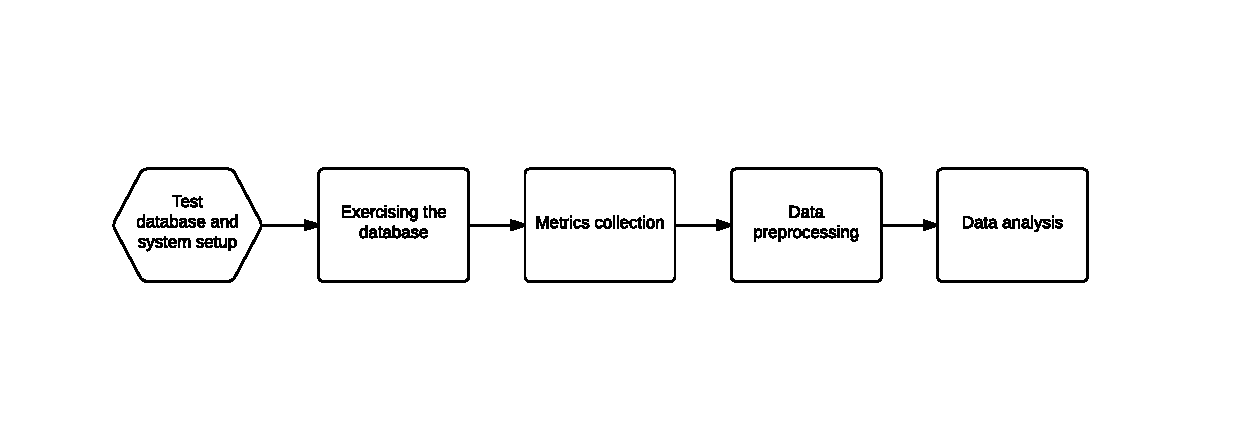
\includegraphics[width=1\textwidth]{approach.pdf}
%	\centering
%	\caption{Approach overview}
%    \label{fig:approach}
%\end{figure} 
%%\includepdf][pages={1}][width=\columnwidth{approach.pdf}

\begin{figure}[!t]
	\centering
	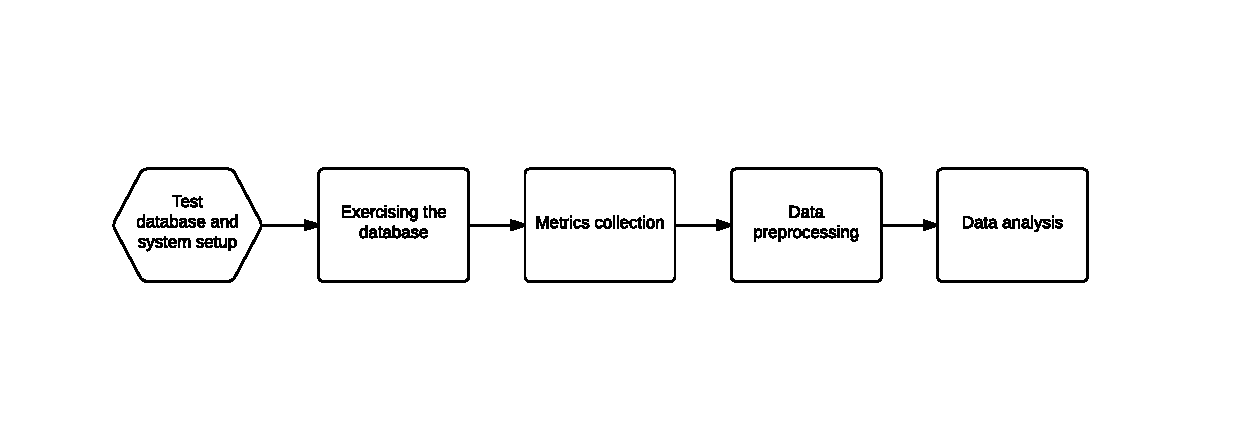
\includegraphics[width=\textwidth]{approach.pdf}
	\caption{Approach Overview}
	\captionsetup{justification=centering}
	\label{fig:Approach}
	
\end{figure}

In this section we discuss the steps in our approach. The primary intention behind our experiment was to observe the performance of the system under test in a virtual environment. Additionally, to analyze whether the metric values depict a similar behavior when compared cross-environment. Once the performance metrics are recorded and processed, we then analyze our results using graphical techniques and regression models. Figure 1 shows the synopsis of our approach.


\subsection{System Setup}
We chose Dell DVD Store (DS2) \cite{delldvd} as our test database. The DVD store is an online e-commerce web application with a multitier architecture, consisting of scripts for MySQL Server, \textit{PHP} web pages and a load driver program written in \textit{C-sharp}. \cite{Shang:2015:ADP:2668930.2688052} \cite{Nguyen:2012:ADP:2188286.2188344} \cite{Nguyen:2012:ADP:2188286.2188344}. \textit{WAMP} \cite{wamp} web application server were used to deploy and exercise the system while the database was set up on MySQL Server 5.6 \cite{mysql}

Based on TPC-W standards \cite{tpcw}, a performance benchmark originally proposed by the Transaction Processing Performance Council, our second subject system under test was also an open source application by CloudScale project \cite{cloudscaleproject} called CloudStore \cite{cloudstore}. Just like DS2, CloudStore serves as online e-commerce website. An online book store, CloudStore is used as a standard in the domain of cloud computing. CloudStore's \textit{JSP} pages were deployed on \textit{Tomcat} \cite{tomcat} and MySQL Server 5.6 \cite{mysql} was used to set up the database. The workload generator was based on scripts written for Apache Jmeter. \cite{apachejmeter}

Our system setup included three machines in a lab environment, Pentium i5 each with an 8GB of memory. To make the systems' configuration identical prior to exercising the subject system, we chose 2 cores and 3GB of memory dedicated to each environment to avoid crashes on the guest operating system. We opted for single tenancy of the guest operating system to avoid any unwanted noise. The first machine was dedicated to the database server, the second machine was dedicated to the web server and the third machine was used to run the load driver.

%\subsection{Exercising the database}
Following the set up of our subject systems on the respective servers, the systems were exercised with an aid of drivers. These drivers generated multi-type web requests and simulated real-time user behavior depending on the input parameters provided by us. We ran our performance tests for numerous hours while recording all the performance metrics generated for varying load applied on our software systems.

The load variation per run was introduced by the number of threads. A higher number of threads represented a higher number of users which would resultantly increase the number of requests per minute and vice-versa. As our study was based on exercising our systems and recording the performance metrics, and not stress testing \cite{stresstesting}, the respected limits were chosen in order to avoid the under-performance of the physical machine and system failure of the virtual machine.

%\subsection{Metrics Collection}
\subsection{Data Transformation}
The values of all the available performance metrics were monitored, recorded every 10 seconds via \textit{perfmon} \cite{windowsperfmon}\cite{perfmon}. \textit{Perfmon} is a system performance monitor used to observe and record performance metrics like CPU utilization, Memory usage and disk IOs. For the reason that our web server and database server were on different machines, we recorded two data sets from two machines monitoring the application process resulting in a data set of 56 metrics. A set of every 6 recorded entries averaged out was labeled as a \textit{single run} representing a minute. This way we had accumulated data from more than 500 runs. We used web server access logs to extract the requests that represented our load. Access logs record every web request that is received by the web server accompanied by the information such as IP addresses, URLs and timestamps \cite{weinberg2003use}. With the help of a script we grouped the web requests per minute. The two data sets were then concatenated and mapped against requests according to the timestamps.

   %\begin{itemize}
   	%\item \textit{User Time}:  	
	 %  	Time the processor takes executing in the user mode.
   	%\item \textit{Privileged time}:
   	 %  	Time the processor takes executing in the privileged mode.
   	%\item \textit{IO Read Operations/Sec}: 
   	 %  	 The rate of issuing of read I/O operations by the process.
   	%\item \textit{IO Read Bytes/Sec}:
   	 %  	The rate at which the process reads bytes from I/O operations.
   	%\item \textit{IO Write Operations/Sec}:
	 %  	   The rate of issuing of write I/O operations by the process.	
   	%\item \textit{IO Write Bytes/sec}:
	 %  	The rate at which the process writes bytes to I/O operations.
   	%\item \textit{Working Set}:
	 %  	Set of memory of pages altered latterly by the process.
   	%\item \textit{Working Set - Private}:
   	%\item \textit{Private Byte}:
	 %  	Bytes allocated to a particular process that cannot be shared.
   %\end{itemize}


\subsection{Data Cleansing and Data Analysis}
Following the data transformation, we used R \cite{R} to derive conclusions for our research questions with the help of Spearman correlation, q-q plots \cite{qqplots}; a graphical technique to detect if two sets of data belong to the same population, Mann-Whitney \textit{U} test \cite{mannwhitney}, and generalized linear regression models (GLM) \cite{SanFranciscoStateUniversity} which are discussed later in detail in section 4. Spearman correlation is used to identify the level of association between two variables while Mann-Whitney \textit{U} test  test is used to verify the hypothesis that if the data sets belong to the same population.
%calculate the absolute deviation in a dataset from the median \cite{brownftest} \textcolor{red}{or instead brown forsythe test. enough already for rq1, discuss}. 
Both these methods do not strictly assume that the ordinal data is normally distributed \cite{spearman} \cite{manutest}. Due to the size of our data, heat maps \cite{heatmaps} were used to visualize the correlations. We chose model-based analysis as they can support the automatic selection and detection of performance abnormalities between heterogeneous environments. \cite{Shang:2015:ADP:2668930.2688052}\cite{Nguyen:2012:ADP:2188286.2188344}. Contrary to the usual practice of ad-hoc selection of certain target performance metrics \cite{heger2013automated} to detect performance regression, we included exhaustive set of all 56 metrics to shape our models. For our linear regression models, we processed our data in two steps. First, we remove any metrics that showed no variance by a R script, for example a metric which has less than 20 unique values \cite{rahm2000data}. Next, we also remove the metrics which have high correlation amongst themselves to remove any \textit{multicollinearity} present \cite{mansfield1982detecting} so that the models do not over fit based on similar predictors(performance metrics) for the load. This approach will also magnify the metric which actually contribute the most to the model. The rationale behind aforementioned steps was to clean up data that may not contribute significantly to the model \cite{Shihab:2010:UIC:1852786.1852792}. 


Once our data was organized our consequent footprint was to build the GLM using the physical and the virtual environment's performance metrics. Our models were built using the load as the dependent variable and the performance metrics as the independent variable i.e. the load is dependent on the change of values of the performance metrics. with the help. We, additionally, trained and tested our models for the same environment before using it cross-environments. This served as the benchmark for lower limit of the prediction percentage error. A model tested for the same environment was validated via ten-fold cross validation \cite{Cross_Validation} \cite{kohavi1995study}. Each fold is based on a random subset of values. The model is trained on 9 folds and tested on the $10^{th}$ fold. This is done 10 times with 10 different subsets of data each time. The accuracy of our models was determined by the percentage error of the predicted load versus the actual load values which was calculated as the absolute difference of the actual and predicted load values with respect to the actual load values.

Based on the results from the GLMs we then investigate about the metrics that are contributing the most and their respective correlation values using heat maps. Heat maps allow us to graphically view, in our case, the individual metrics and their correlation values. 